%versi 2 (8-10-2016)
\chapter{Landasan Teori}
\label{chap:teori}

Bab ini membahas tentang landasan teori yang akan digunakan dalam skripsi ini yang diambil dari dua sumber, yaitu ''CodeIgniter Documentation'' karya British Columbia Institute of Technology ~\cite{bcit:17:cidoc} dan ''Sharif Judge Documentation'' karya Mohammad Javad Naderi ~\cite{mjnaderi:14:sharifjudgedoc}.

\section{\textit{CodeIgniter}}
\label{sec:codeigniter} 
 
\textit{CodeIgniter} merupakan sebuah \textit{framework} bagi pengguna yang ingin membangun aplikasi web menggunakan PHP. Tujuan utamanya adalah memungkinkan para pengguna mengembangkan proyek-proyek menjadi lebih cepat dibandingkan menulis kode dari awal. \textit{Framework} ini memiliki banyak libary untuk tugas-tugas yang biasa diperlukan, serta antarmuka dan struktur logis yang sederhana untuk mengakses library ini. CodeIgniter membuat para pengguna lebih fokus pada proyek dengan meminimalkan jumlah kode yang dibutuhkan untuk tugas yanf diberikan~\cite{bcit:17:cidoc}. \\

Beberapa keunggulan dari \textit{CodeIgniter} yaitu:
\begin{itemize}
	\item \textit{Framework} yang Ringan \\
		Inti dari sistem CodeIgniter hanya membutuhkan \textit{library} yang kecil. Hal ini sangat berbeda dengan framework lain yang membutuhkan \textit{resource} yang lebih. \textit{Library} tambahan dimuat secara dinamis atau sesuai dengan permintaan sehingga sistem dapat berjalan cepat.
	\item Menggunakan Konsep M-V-C \\
		\textit{CodeIgniter} menggunakan pendekatan \textit{Model-View-Controller} yang memungkinkan pemisahan anatara logika dan presentasi.
	\item Menghasilkan \textit{Clean URLs} \\
		\textit{URL} yang dihasilkan oleh  \textit{CodeIgniter} berish dan \textit{search-engine friendly}. \textit{CodeIgniter} menggunakan pendekatan \textit{segment-based} seperti: \\example.com/news/article/345
	\item \textit{Packs a Punch} \\
		\textit{CodeIgniter} dilengkapi dengan \textit{library} yang umumnya diperlukan untuk tugas pengembangan web seperti mengakses database, mengirim email, memvalidasi data \textit{form}, menjaga \textit{session}, memanipulasi gambar, bekerja dengan \textit{XML-RPC} data dan masih banyak lagi.
	\item \textit{Extensible} \\
		Sistem dapat dengan mudah diperluas dengan menggunakan \textit{library} pengguna, \textit{helper}, atau melalui \textit{class extensions} dan \textit{system hooks}.
	\item Tidak Membutuhkan \textit{Template Engine} \\
		\textit{CodeIgniter} dilengkapi dengan \textit{template parser} sederhana yang dapat digunakan secara opsional. \textit{Template Engine} tidak dapat menandingi kinerja dari \textit{native} PHP. Sintak yang harus dipelajari untuk menggunakan \textit{Template Engine} biasanya lebih mudah dari mempelajari dasar-dasar PHP. Perhatikan potongan kode PHP di bawah ini: \\
		\begin{lstlisting}[backgroundcolor = \color{lightgray}]
		<ul>
		<?php foreach ($addressbook as $name):?>
		<li><?=$name?></li>
		<?php endforeach; ?>
		</ul>
		\end{lstlisting}
		
		Sangat berlawanan dengan \textit{pseudo-code} yang digunakan oleh \textit{Template Engine}: \\
		\begin{lstlisting}[backgroundcolor = \color{lightgray}]
		<ul>
		{foreach from=$addressbook item="name"}
		<li>{$name}</li>
		{/foreach}
		</ul>
		\end{lstlisting}
		Terlihat \textit{Template Engine} sedikit lebih bersih, namun harus ditukar dengan performa yang kurang baik karena \textit{pseudo-code} harus dikonversi kembali menjadi PHP. Salah satu tujuan dari \textit{CodeIgniter} adalah performa maksimal, oleh karena itu \textit{CodeIgniter} tidak menggunakan \textit{Template Engine}.
	\item Dokumentasi yang Baik \\
		Dokumentasi merupakan salah satu bagian terpenting dari kode itu sendiri. \textit{CodeIgniter} berkomitmen membuat kode yang sangat bersih dan terdokumentasi dengan baik. 
\end{itemize}

\subsection{Fitur-fitur CodeIgniter}
Berikut beberapa fitur utama yang terdapat pada \textit{framework CodeIgniter} seperti:
\begin{itemize}
	\item Sistem berbasis \textit{MVC}
	\item \textit{Framework} yang ringan
	\item \textit{Database Class} yang lengkap dengan dukungan untuk beberapa platform
	\item Dukungan \textit{query builder} untuk database
	\item \textit{Form} dan validasi data
	\item Keamanan dan \textit{XSS Filtering}
	\item \textit{Session Management}
	\item \textit{Email Sending Class}
	\item \textit{Image Manipulation Library}
	\item \textit{File Uploading Class} 
	\item \textit{Calendaring Class}
	\item \textit{Unit Testing Class}
\end{itemize}

\subsection{\textit{Flow Chart} Aplikasi}
Gambar~\ref{fig:flow} menunjukan bagaimana data mengalir ke seluruh sistem~\cite{bcit:17:cidoc}:
\begin{figure}[H]
	\centering  
	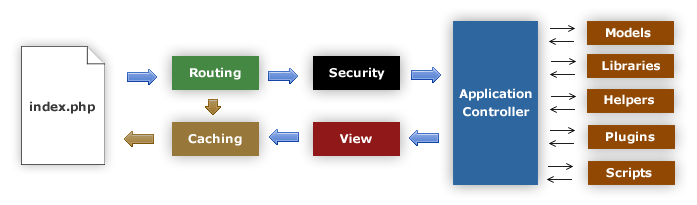
\includegraphics[scale=1]{appflowchart}  
	\caption[\textit{Flow Chart} Aplikasi]{\textit{Flow Chart} Aplikasi} 
	\label{fig:flow} 
\end{figure} 

\begin{enumerate}
	\item File \textit{index.php} berfungsi sebagai \textit{front controller} dan menginisialisasi \textit{resource} utama yang dibutuhkan untuk menjalankan \textit{CodeIgniter}.
	\item \textit{Router} memeriksa \textit{HTTP request} untuk menentukan apa yang harus dilakukan.
	\item Jika terdapat \textit{file cache}, maka akan langsung dikirimkan ke \textit{browser}.
	\item \textit{HTTP request} dan data pengguna yang dikirim akan terlebih dahulu disaring untuk alasan keamanan. \textit{Application controller} akan dimuat setelah proses penyaringan selesai.
	\item \textit{Controller} akan memuat \textit{model, core libraries, helpers} dan \textit{resource} lain yang dibutuhkan untuk memproses permintaan khusus.
	\item \textit{View} akan di \textit{render} kemudian dikirim ke web \textit{browser}. Jika proses \textit{caching} diaktifkan, maka \textit{View} akan di \textit{cache} terlebih dahulu sehingga permintaan berikutnya dapat dilayani.
\end{enumerate}

\subsection{\textit{Model-View-Controller}}
\textit{CodeIgniter} merupakan \textit{framework} yang menggunaakan pola pengembangan \textit{Model-View-Controller}. \textit{MVC} adalah pendekatan perangkat lunak yang memisahkan logika aplikasi dari presentasi. Hal tersebut memungkinkan halaman web pengguna memiliki \textit{scripting} yang minimal karena presentasi terpisah dari \textit{scripting} PHP~\cite{bcit:17:cidoc}. \\
\begin{itemize}
	\item \textit{Model} merepresentasikan bagian struktur data pengguna. Biasanya kelas \textit{Model} akan berisikan fungsi-fungsi yang membantu pengguna untuk mengambil, menyimpan, dan memperbarui informasi pada database.
	\item \textit{View} merupakan informasi yang akan ditampilkan kepada pengguna. Umumnya \textit{View} merupakan sebuah halaman web, namun pada \textit{CodeIgniter}, \textit{View} dapat berupa bagian-bagian halaman seperti \textit{header} atau \textit{footer}. Selain itu \textit{View} juga dapat berupa halaman \textit{RSS} atau jenis "halaman" lainnya.
	\item \textit{Controller} berfungsi sebagai perantara antara \textit{Model}, \textit{View}, dan \textit{resource} lain yang dibutuhkan untuk memproses \textit{HTTP request} dan menghasilkan halaman web.
\end{itemize}
\textit{CodeIgniter} memiliki pendekatan yang cukup fleksibel terhadap \textit{MVC} karena \textit{Model} tidak selalu diperlukan. Para pengguna dapat membangun aplikasi minimal  menggunakan \textit{Controller} dan \textit{View}. Hal tersebut dapat dilakukan jika pengguna tidak memerlukan adanya pemisahan tambahan atau pengguna merasa bahwa mempertahankan sebuah \textit{Model} membutuhkan kompleksitas yang lebih tinggi~\cite{bcit:17:cidoc}. 

\subsection{Desain dan Tujuan Arsitektur}
Dari sudut pandang teknis, dan arsitektural, CodeIgniter dibuat dengan tujuan sebagai berikut:
\begin{itemize}
	\item \textit{Dynamic Instation} \\
	Dalam \textit{CodeIgniter}, komponen dimuat dan rutinitas dieksekusi hanya jika diminta. Tidak ada asumsi yang dibuat oleh sistem tentang apa yang mungkin diperlukan di luar resource utama, sehingga sistem ini sangat ringan secara \textit{default}. \textit{Event}, \textit{Controller} dan \textit{View} yang pengguna rancang akan menentukan apa yang dipanggil.
	\item \textit{Loose Coupling} \\
	\textit{Coupling} adalah sejauh mana komponen-komponen dari sistem saling mengandalkan satu sama lain. Semakin sedikit komponen yang bergantung satu sama lain, maka komponen tersebut lebih dapat digunakan kembali dan sistem menjadi fleksibel. Tujuan dari \textit{framework} ini adalah sistem yang sangat longgar (\textit{very loosely coupled system}).
	\item \textit{Component Singularity} \\
	\textit{Singularity} adalah sejauh mana komponen memiliki tujuan yang difokuskan secara sempit. Dalam CodeIgniter, setiap kelas dan fungsinya sangat otonom. Hal tersebut memungkinkan fungsi dapat berjalan secara maksimal.
\end{itemize}

CodeIgniter merupakan sistem yang loosely coupled dengan singularitas komponen yang tinggi (\textit{dynamically instantiated}). Codeigniter berusaha untuk sederhana, fleksible, dan kinerja tinggi dengan paket yang sekecil mungkin ~\cite{bcit:17:cidoc}.

\section{\textit{Sharif Judge}}
\label{sec:sharifjudge} 

\textit{Sharif Judge} adalah \textit{grader} otomatis yang mampu menilai ketepatan serta performansi program yang dikumpulkan mahasiswa. Perangkat lunak ini diciptakan oleh Mohammad Javad Naderi dan bersifat \textit{open source}. \textit{Web Interface} perangkat lunak ini ditulis menggunakan PHP ()\textit{framework CodeIgniter}) dan \textit{backend} menggunakan \textit{BASH} \cite{mjnaderi:14:sharifjudge}.
Selain sebagai \textit{grader} otomatis, \textit{Sharif Judge} juga memiliki beberapa fitur lainnya seperti:
\begin{itemize}
	\item Beberapa peran pengguna (\textit{admin, head instructor, instructor, student})
	\item Sandboxing (belum diterpakan untuk \textit{phyton})
	\item Deteksi kecurangan (mendeteksi kode yang mirip) menggunakan \textit{Moss}
	\item Pengaturan untuk menilai keterlambatan pengiriman
	\item Antrian Pengiriman
	\item Mengunduh hasil dalam bentuk \textit{file excel}
	\item Mengunduh kode yang telah dikirim dalam bentuk \textit{file zip}
	\item Metode "\textit{Output Comparison}" dan "\textit{Tester Code}" untuk memeriksa kebenaran dari hasil keluaran.
	\item Menambahakan beberapa pengguna sekaligus
	\item Diskripsi Masalah (\textit{PDF/Markdown/HTML})
	\item Penilaian ulang (\textit{rejudge})
	\item Papan nilai
	\item Notifikasi
\end{itemize}

\subsection{Instalasi}
Untuk menjalankan Sharif Judge membutuhkan sebuah \textit{server Linux} dengan persyaratan berikut:
\begin{itemize}
	\item \textit{Webserver} menjalankan PHP versi 5.3 atau yang lebih baru
	\item Pengguna harus dapat menjalankan php dari \textit{command line}. Pada \textit{Ubuntu}, pengguna perlu meginstal paket \textit{php5-cli}
	\item \textit{Mysql database} (dengan ekstensi \textit{mysqli} untuk PHP) atau \textit{PostgreSql database}
	\item PHP harus memiliki akses untuk menjalankan \textit{shell commands} menggunakan fungsi \textit{shell\textunderscore exec}. Contohnya seperti \textit{command} di bawah ini: 
		\begin{lstlisting}[backgroundcolor = \color{lightgray}]
		echo shell_exec("php -v");
		\end{lstlisting}
	\item Perkakas yang digunakan untuk \textit{compiling} dan menjalankan kode yang dikumpulkan (\textit{gcc, g++, javac, java, python2, python3 commands})
	\item \textit{Perl} lebih baik diinstal untuk ketepatan waktu, batas memori dan memaksimalkan batas ukuran pada \textit{output} kode yang dikirimkan
\end{itemize}


Jika persyaratan di atas telah terpenuhi, maka akan masuk tahap instalasi sebagai berikut:
\begin{itemize}
	\item Mengunduh versi terakhir dari Sharif Judge dan \textit{unpack} hasil download di direktori \textit{public html}
	\item (Pilihan) Pindahkan folder \textit{system} dan \textit{application} keluar dari \textit{public directory} dan
	masukan \textit{path} lengkap di \textit{file index.php} 
	\begin{lstlisting}[backgroundcolor = \color{lightgray}]
	$system_path = '/home/mohammad/secret/system';
	$application_folder = '/home/mohammad/secret/application';
	\end{lstlisting}
	\item Buat sebuah \textit{Mysql} atau \textit{PostgreSql} database untuk Sharif Judge. Jangan menginstall paket koneksi database untuk \textit{C/C++, Java}, atau \textit{Python}
	\item Atur pengaturan koneksi database di file \textit{application/config/database.php}. Pengguna dapat menggunakan awalan untuk nama tabel.
	\begin{lstlisting}[backgroundcolor = \color{lightgray}]
	/*  Enter database connection settings here:  */
	'dbdriver' => 'postgre',    // database driver (mysqli, postgre)
	'hostname' => 'localhost',  // database host
	'username' => `,           // database username
	'password' => `,           // database password
	'database' => `,           // database name
	'dbprefix' => 'shj_',       // table prefix
	/**********************************************/
	\end{lstlisting}
	\item Buat \textit{application/cache/Twig} dapat ditulis oleh PHP
	\item Buka halaman utama \textit{Sharif Judge} pada web \textit{browser} dan ikuti proses instalasi berikutnya
	\item \textit{Log in} menggunakan akun \textit{admin}
	\item Pindahkan folder \textit{tester} dan \textit{assigments} di luar \textit{public directory} lalu simpan \textit{path} lengkap di halaman \textit{Settings}. Dua folder tersebut harus dapat ditulis oleh PHP. File-file yang diserhkan akan disimpan di folder \textit{assigments} sehingga tidak dapat diakses publik.
\end{itemize}

\subsection{\textit{Clean URLs}}
Secara \textit{default}, \textit{index.php} merupakan bagian dari seluruh \textit{urls} yang ada pada \textit{Sharif Judge} seperti: 
\begin{lstlisting}[backgroundcolor = \color{lightgray}]
http://example.mjnaderi.ir/index.php/dashboard
http://example.mjnaderi.ir/index.php/users/add
\end{lstlisting}
Pengguna dapat menghilangkan \textit{index.php} dan memiliki \textit{urls} yang baik jika sistem pengguna mendukung aturan \textit{rewrite} seperti:  
\begin{lstlisting}[backgroundcolor = \color{lightgray}]
http://example.mjnaderi.ir/dashboard
http://example.mjnaderi.ir/users/add
\end{lstlisting}

Untuk memungkinkan \textit{clean urls}, ubah isi file \textit{.htaccess2} menjadi \textit{.htaccess} yang berlokasi di direktori utama \textit{Sharif Judge}.
Berikut isi file \textit{.htaccess2}: 
\begin{lstlisting}[backgroundcolor = \color{lightgray}]
# You also need to change 
# $config['index_page'] = 'index.php';
# to
# $config['index_page'] = '';
# in application/config/config.php
# in order to enable clean urls.

RewriteEngine on
RewriteCond $1 !^(index\.php|assets|robots\.txt)
RewriteRule ^(.*)$ index.php?/$1 [L]
\end{lstlisting}
Lalu buka file \textit{application/config/config.php} dan ubah  
\begin{lstlisting}[backgroundcolor = \color{lightgray}]
$config['index_page'] = 'index.php';
\end{lstlisting}
menjadi
\begin{lstlisting}[backgroundcolor = \color{lightgray}]
$config['index_page'] = '';
\end{lstlisting}

\subsection{\textit{Users}}
Pada \textit{Sharif Judge}, pengguna dikelompokan menjadi 4 yaitu \textit{Admins, Head Instructor, Instructor, }dan \textit{Students}
Tabel~\ref{tab:userrole} menunjukan \textit{level} para pengguna.

\begin{table}[H] %atau h saja untuk "kira kira di sini"
	\centering 
	\caption{\textit{User Roles Table}}
	\label{tab:userrole}
	\begin{tabular}{cc}
		\toprule
		\textit{User Role} & \textit{User Level} \\
		
		\midrule
		\textit{Admin} & 3 \\
		\textit{Head Instructor} & 2 \\
		\textit{Instructor} & 1 \\
		\textit{Student} & 0 \\
		
		\bottomrule
		
	\end{tabular} 
\end{table}

Setiap pengguna memiliki aksi yang berbeda-beda. Aksi yang dapat dilakukan para pengguna akan diseaikan dengan level masing-masing. Perhatikan tabel~\ref{tab:useraction} berikut:
\begin{table}[H] %atau h saja untuk "kira kira di sini"
	\centering 
	\caption{\textit{Permission Table}}
	\label{tab:useraction}
	\begin{tabular}{ccccc}
		\toprule
		Aksi & \textit{Admin} & \textit{Head Instructor} & \textit{Instructor} & \textit{Student} \\
		
		\midrule
		Mengubah \textit{Settings} & BISA & GB & GB & GB \\
		Mengubah \textit{Settings} & BISA & GB & GB & GB \\
		Mengubah \textit{Settings} & BISA & GB & GB & GB \\
		Mengubah \textit{Settings} & BISA & GB & GB & GB \\
		
		\bottomrule
		
	\end{tabular} 
\end{table}
\dtext{11-12} 

\section{\LaTeX}
\label{sec:latex}

Mengapa menggunakan \LaTeX{} untuk buku skripsi dan apa keunggulan/kerugiannya bagi mahasiswa dan pembuat template. 

\dtext{13-14}


\section{Template Skripsi FTIS UNPAR}
\label{sec:template}
 
Akan dipaparkan bagaimana menggunakan template ini, termasuk petunjuk singkat membuat referensi, gambar dan tabel.
Juga hal-hal lain yang belum terpikir sampai saat ini. 
 
\dtext{15-16}

\subsection{Tabel}  
Berikut adalah contoh pembuatan tabel. 
Penempatan tabel dan gambar secara umum diatur secara otomatis oleh \LaTeX{}, perhatikan contoh di file bab2.tex untuk melihat bagaimana cara memaksa tabel ditempatkan sesuai keinginan kita.

Perhatikan bawa berbeda dengan penempatan judul gambar gambar, keterangan tabel harus diletakkan di atas tabel!!
Lihat Tabel~\ref{tab:contoh1} berikut ini:

\begin{table}[H] %atau h saja untuk "kira kira di sini"
	\centering 
	\caption{Tabel contoh}
	\label{tab:contoh1}
	\begin{tabular}{cccc}
		\toprule
		& $v_{start}$ & $\mathcal{S}_{1}$ & $v_{end}$\\

		\midrule
		$\tau_{1}$ & 1 & 12& 20\\
		$\tau_{2}$ & 1 &  & 20\\
		$\tau_{3}$ & 1 & 9 & 20\\
		$\tau_{4}$ & 1 &  & 20\\

		\bottomrule
		
	\end{tabular} 
\end{table}
Tabel~\ref{tab:cthwarna1} dan Tabel~\ref{tab:cthwarna2} berikut ini adalah tabel dengan sel yang berwarna dan ada dua tabel yang bersebelahan. 
\begin{table}[H]
	\begin{minipage}[c]{0.49\linewidth}
		\centering
		\caption{Tabel bewarna(1)}
		\label{tab:cthwarna1}
		\begin{tabular}{ccccc}
			\toprule
			 & $v_{start}$ & $\mathcal{S}_{2}$ & $\mathcal{S}_{1}$ & $v_{end}$\\
			
			\midrule
			$\tau_{1}$ & 1 & 5 \cellcolor{green}& 12& 20\\
			$\tau_{2}$ & 1 & 8 \cellcolor{green}& & 20\\
			$\tau_{3}$ & 1 & 2/8/17 \cellcolor{green}& 9 & 20\\
			$\tau_{4}$ & 1 & \cellcolor{red}& & 20\\
			
			\bottomrule

		\end{tabular}
	\end{minipage}
	\begin{minipage}[c]{0.49\linewidth}
		
		\centering 
		\caption{Tabel bewarna(2)}
		\label{tab:cthwarna2}
		\begin{tabular}{ccccc}
			\toprule
			 & $v_{start}$ & $\mathcal{S}_{1}$ & $\mathcal{S}_{2}$ & $v_{end}$\\
			
			\midrule
			$\tau_{1}$ & 1 & 12& 5 \cellcolor{red} &20\\
			$\tau_{2}$ & 1 &  &  8 \cellcolor{green} &20\\
			$\tau_{3}$ & 1 & 9 & 2/8/17 \cellcolor{green} &20\\
			$\tau_{4}$ & 1 &   & \cellcolor{red} &20\\
			
			\bottomrule
		
		\end{tabular}
	\end{minipage}
\end{table}

 
\subsection{Kutipan}
\label{subs:kutipan} 
Berikut contoh kutipan dari berbagai sumber, untuk keterangan lebih lengkap, silahkan membaca file referensi.bib yang disediakan juga di template ini.
Contoh kutipan:
\begin{itemize}
	\item Buku:~\cite{berg:08:compgeom} 
	\item Bab dalam buku:~\cite{kreveld:04:GIS}
	\item Artikel dari Jurnal:~\cite{buchin:13:median}
	\item Artikel dari prosiding seminar/konferensi:~\cite{kreveld:11:median}
	\item Skripsi/Thesis/Disertasi:~\cite{lionov:02:animasi}~\cite{wiratma:10:following}~\cite{wiratma:22:later}
	\item Technical/Scientific Report:~\cite{kreveld:07:watertight}
	\item RFC (Request For Comments):~\cite{RFC1654}
	\item Technical Documentation/Technical Manual:~\cite{Z.500}~\cite{unicode:16:stdv9}~\cite{google:16:and7}
	\item Paten:~\cite{webb:12:comm}
	\item Tidak dipublikasikan:~\cite{wiratma:09:median}~\cite{lionov:11:cpoly}
	\item Laman web:~\cite{erickson:03:cgmodel}  
	\item Lain-lain:~\cite{agung:12:tango}
\end{itemize}    
  
\subsection{Gambar}

Pada hampir semua editor, penempatan gambar di dalam dokumen \LaTeX{} tidak dapat dilakukan melalui proses {\it drag and drop}.
Perhatikan contoh pada file bab2.tex untuk melihat bagaimana cara menempatkan gambar.
Beberapa hal yang harus diperhatikan pada saat menempatkan gambar:
\begin{itemize}
	\item Setiap gambar {\bf harus} diacu di dalam teks (gunakan {\it field} {\sc label})
	\item {\it Field} {\sc caption} digunakan untuk teks pengantar pada gambar. Terdapat dua bagian yaitu yang ada di antara tanda $[$ dan $]$ dan yang ada di antara tanda $\{$ dan $\}$. Yang pertama akan muncul di Daftar Gambar, sedangkan yang kedua akan muncul di teks pengantar gambar. Untuk skripsi ini, samakan isi keduanya.
	\item Jenis file yang dapat digunakan sebagai gambar cukup banyak, tetapi yang paling populer adalah tipe {\sc png} (lihat Gambar~\ref{fig:ularpng}), tipe {\sc jpg} (Gambar~\ref{fig:ularjpg}) dan tipe {\sc pdf} (Gambar~\ref{fig:ularpdf})
	\item Besarnya gambar dapat diatur dengan {\it field} {\sc scale}.
	\item Penempatan gambar diatur menggunakan {\it placement specifier} (di antara tanda  $[$ dan $]$ setelah deklarasi gambar.
	Yang umum digunakan adalah {\bf H} untuk menempatkan gambar {\bf sesuai} penempatannya di file .tex atau  {\bf h} yang berarti "kira-kira" di sini. \\
	Jika tidak menggunakan {\it placement specifier}, \LaTeX{} akan menempatkan gambar secara otomatis untuk menghindari bagian kosong pada dokumen anda.
	Walaupun cara ini sangat mudah, hindarkan terjadinya penempatan dua gambar secara berurutan. 	
	\begin{itemize}
		\item Gambar~\ref{fig:ularpng} ditempatkan di bagian atas halaman, walaupun penempatannya dilakukan setelah penulisan 3 paragraf setelah penjelasan ini.
		\item Gambar~\ref{fig:ularjpg} dengan skala 0.5 ditempatkan di antara dua buah paragraf. Perhatikan penulisannya di dalam file bab2.tex!
		\item Gambar~\ref{fig:ularpdf} ditempatkan menggunakan {\it specifier} {\bf h}.
	\end{itemize}
\end{itemize}
 
\dtext{17-18}
\begin{figure} 
	\centering  
	\includegraphics[scale=1]{ular-png}  
	\caption[Gambar {\it Serpentes} dalam format png]{Gambar {\it Serpentes} dalam format png} 
	\label{fig:ularpng} 
\end{figure} 

\dtext{19-20}
\begin{figure}[H]
	\centering  
	\includegraphics[scale=0.5]{ular-jpg}  
	\caption[Ular kecil]{Ular kecil} 
	\label{fig:ularjpg} 
\end{figure} 
\dtext{21-22}

\begin{figure}[ht] 
	\centering  
	\includegraphics[scale=1]{ular-pdf}  
	\caption[ {\it Serpentes} betina]{ {\it Serpentes} jantan} 
	\label{fig:ularpdf} 
\end{figure} 
 
